\documentclass[a4paper,10pt,onecolumn,oneside,openany]{jsbook}

\usepackage{amsmath,amssymb}
\usepackage{bm}
%\usepackage{graphicx}
\usepackage[dvipdfmx]{graphicx}
\usepackage{verbatim}
\usepackage{wrapfig}
\usepackage{ascmac}
\usepackage{makeidx}
\usepackage[toc,page]{appendix}
\usepackage{docmute}
\usepackage{array}

\makeindex

\setlength{\textwidth}{155truemm}
\setlength{\fullwidth}{\textwidth}
\setlength{\oddsidemargin}{27truemm}
\addtolength{\oddsidemargin}{-1truein}

\setlength{\topmargin}{25truemm}
\setlength{\textheight}{237truemm}
\addtolength{\topmargin}{-1truein}

\def\linesparpage#1{\baselineskip=\textheight
   \divide\baselineskip by #1}
\def\kcharparline#1{
   \ifx\xkanjiskip\undefined

   \jintercharskip 0mm plus 0.2mm minus 0.2mm
   \else

   \xkanjiskip 0mm plus 0.2mm minus 0.2mm
   \fi
   \settowidth{\textwidth}{あ}
   \multiply\textwidth by #1}

\setcounter{tocdepth}{2}

\begin{document}

\linesparpage{32}
\kcharparline{40}


\begin{titlepage}
\begin{center}
{\huge 卒業論文 \\ }
\vspace*{150truept}
{\huge 超電導接合における二次元電子中の電気伝導}\\
\vspace{100truept}
{\large 指導教員:大岩 顕 教授 \\ }
\vspace{30truept}
{\large 2018/2/17}\\%%\hspace{15pt}
{\large 学籍番号 \hspace{15pt} 08D14160}\\
{\large 氏名 \hspace{15pt} 吉原 拓哉}\\
\vspace{100truept}
{\huge 大阪大学工学部電子情報工学科}\\
{\huge 量子電子デバイスコース}\\
{\huge 量子システム創成研究分野}\\
\end{center}
\end{titlepage}

\tableofcontents
\mainmatter

\makeatletter
\newcommand{\figcaption}[1]{\def\@captype{figure}\caption{#1}}
\newcommand{\tblcaption}[1]{\def\@captype{table}\caption{#1}}
\makeatother

\documentclass[a4paper,10pt,onecolumn,oneside,openany]{jsbook}

\usepackage{amsmath,amssymb}
\usepackage{bm}
%\usepackage{graphicx}
\usepackage[dvipdfmx]{graphicx}
\usepackage{verbatim}
\usepackage{wrapfig}
\usepackage{ascmac}
\usepackage{makeidx}
\usepackage[toc,page]{appendix}
\usepackage{array}
\usepackage{docmute}
\usepackage{wrapfig}
\makeatletter
\newcommand{\subsubsubsection}{\@startsection{paragraph}{4}{\z@}%
  {1.0\Cvs \@plus.5\Cdp \@minus.2\Cdp}%
  {.1\Cvs \@plus.3\Cdp}%
  {\reset@font\sffamily\normalsize}
}
\makeatother
\usepackage[hang,small,bf]{caption}
\usepackage[subrefformat=parens]{subcaption}
\captionsetup{compatibility=false}

\makeindex
\setlength{\textwidth}{155truemm}
\setlength{\fullwidth}{\textwidth}
\setlength{\oddsidemargin}{27truemm}
\addtolength{\oddsidemargin}{-1truein}

\setlength{\topmargin}{25truemm}
\setlength{\textheight}{237truemm}
\addtolength{\topmargin}{-1truein}

\def\linesparpage#1{\baselineskip=\textheight
   \divide\baselineskip by #1}
\def\kcharparline#1{
   \ifx\xkanjiskip\undefined

   \jintercharskip 0mm plus 0.2mm minus 0.2mm
   \else

   \xkanjiskip 0mm plus 0.2mm minus 0.2mm
   \fi
   \settowidth{\textwidth}{��}
   \multiply\textwidth by #1}

\setcounter{tocdepth}{2}

\begin{document}

\linesparpage{32}
\kcharparline{40}
\chapter{������@}
\section{�����쐻}
\subsection{GaAsHEMT��\��}
�{�����Ŏg�p������‚͏Z�F�d�C�H�Ɗ�����А���GaAsAlGaAs���ړ��x�񎟌��d�q(No.501672HEMT)
��‚�p�����B�����\�͈ȉ��̒ʂ�ł���B�܂��A�l�[�q����ŗp�����_�~�[��‚̓o���N��GaAs��‚ł���B
\newcolumntype{I}{!{\vrule width 1.2pt}}
\newlength\savedwidth
\newcommand{\wcline}[1]{\noalign{\global\savedwidth\arrayrulewidth\global\arrayrulewidth 1.2pt} \cline{#1}
\noalign{\global\arrayrulewidth\savedwidth}}
\begin{table}[htb]
  \begin{center}
    \caption{�{�����ɗp������‚̓����\}
    \begin{tabular}{|cIc|c|cIc|} \hline
      �\�� & �h�[�s���O�Z�x(cm${}^\text{-3}$) & �h�[�p���g & ����(\AA) & Al�g�� \\ \hline
      GaAs & �[ & �[ & 50 & �[ \\\hline
      N-AlGaAs & 1.0E18 & Si & 650 & 0.265 \\\wcline{1-5}
      AlGaAs& �[ & �[ & 300 & 0.265 \\\hline
      GaAs & �[ & �[ & 8000 & �[ \\\hline
      \multicolumn{1}{|cI}{GaAs���}& \multicolumn{4}{c|}{3^{n}\mbox{GaAs�@���d�^:���≏�@����:600}\mu \mbox{m�@���a:76mm�@�ʕ���:(100)}\pm 0.5^{\circ}}\\ \hline
    \end{tabular}
    \label{tab:price}
  \end{center}
\end{table}

\subsection{�����̃f�U�C��}
2�����d�q�n�ł̒��`���𒲂ׂ邽�߂̓K�؂Ȏ����\����݌v�����B
�}\ref{fig:abstsub}�̂悤�Ƀ��T��ɐ�$\mu$�̊Ԋu��������
�Q�‚̒��`���̂����������A�I�[�~�b�N�ڐG�ɂ��Q�����d�q�փR���^�N�g���Ƃ�
���Ƃ��ł��ASNS�ڍ����`���ł���B����ɂ��A���`���M���b�v���O�ɑ��d���˓�
�ɋN����������I�ȓd���d������������A�l�X�ȏ�񂪓�����B
%���Ƃ�HEMT��dummy�ɂ‚��Ēlj�
\begin{figure}[htbp]
  \begin{center}
    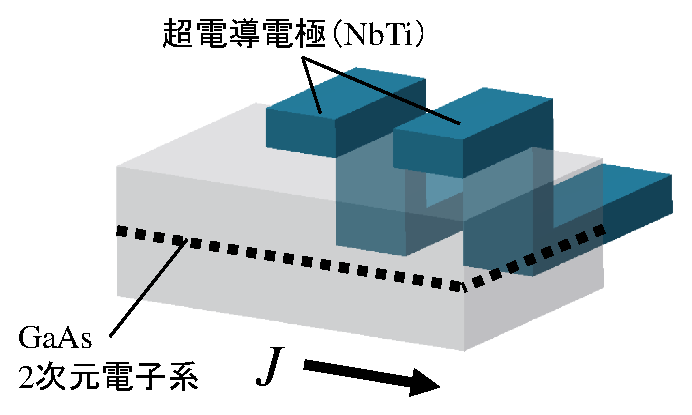
\includegraphics[width=10cm]{../images/abstsub0.eps}
  \end{center}
  \caption{�쐬����SNS�ڍ��̊T���}}
   \label{fig:abstsub}
\end{figure}

\subsection{���׉��H�v���Z�X}
��{�I��CAD�}�`�\�t�g��p���ăi�m�X�P�[���̓d�Ƀp�^�[����݌v���A
�d�q�����\�O���t�B�[�A�t�H�g���\�O���t�B�[�̋Z�p��p���ĘI�����A������ɁA
�E�F�b�g�G�b�`���O�܂��͓d�q���������u��p���ċ����d�ɂ�����������v���Z�X���J��Ԃ����ƂŎ����쐻���s�����B\\
�ȉ��Ɋe�v���Z�X�ɋ��ʂ����{�I�ȍH�����q�ׂ��̂��A�����쐻�̍H�����������B\\
\subsubsection{��{�I�ȍH��}
\subsubsubsection{1. ����}
    �A�Z�g��2��AIPA1��e�T�����“���A���f�K�X�Ŋ��������A110���̃z�b�g�v���[�g��
    10���Ԋ���������B
\subsubsubsection{2.���W�X�g�h�z}
    ���W�X�g����‚ɓH�����A�X�s���R�[�^�[��p���ă��W�X�g�̌������ψ�ɂ���B
    �X�s���R�[�^�[�̏����͎��̒ʂ�B(500rpm 5�b�Aslope 5�b�A4000rpm 50�b�Aslope 5�b�Aend)
    ���̌�A��‚̗��ɂ‚������W�X�g���A�Z�g���Ő@���Ƃ�B
\subsubsubsection{3.�v���x�[�L���O}
 ���W�X�g���ʼn������邽�߂Ƀz�b�g�v���[�g�ʼn��M����B�e���W�X�g�ɂ���������͈ȉ��̒ʂ�B(PMMA 180�� 3���AS1813 115�� 3���ALOR 180�� 5��)
\subsubsubsection{4.�I��}
    ���d���d�ɓ��ׂ̍����p�^�[���͓d�q���`�摕�u(�ȉ�EB)�ŘI�����A����ȊO�̑傫�ȃp�^�[����LED�`�摕�u(�ȉ�LED)�ŕ`����s�����B
\subsubsubsection{5.����}
    �I�����ꂽ���W�X�g�������t�ɐZ���邱�Ƃɂ�蕪�����Ď�菜�����B�{�����ł́APMMA�̌����ɂ̓��`���C�\�u�`���P�g��(MIBK)
    ��IPA��1��2�̊����Ŕ��߂����̂�10�x�ɗ�₵�A2�����x����A���̌�AIPA��1������A�������~�߂�B
    �܂�LOR��S1813��2�w���W�X�g�ł�NMD��90�`120�b�ԓ��ꂽ��A�����̓������r�[�J�[�ɂ����点�A������x�􂢗�������A
    �ʂ̏����̓������r�[�J�[��1������A�������~�߂�B
  \subsubsubsection{6.����}
    �܂��A�\�ʂɗL�@�����t���Ă���”\��������̂ŁA10$\%$�̊󗰎_��30�b����A���̌㏃����3�`5�����x��򂵂��B
  �@�^���Ԃ̏������u���Ō����ɓd�q���𓖂āA�����v�ŏ��]�̖����ɂȂ�܂Ō��������������B
  \subsubsubsection{7.�G�b�`���O}
�@  ��‚̃G�b�`���O�͑S�ăE�F�b�g�G�b�`���O��p�����B�E�F�b�g�G�b�`���O�ł͊�‚��G�b�`���O�t
    (H${}_\text{2}$SO${}_\text{4}$:H${}_\text{2}$O${}_\text{2}$:H${}_\text{2}$O��1:8:160)�ɓ���A�P������
    10���ɕۂ��Ȃ���G�b�`���O���s���B�K���Ȏ��ԂŊ�‚����o���A�ڐG���̒i���v�Ń��W�X�g�\�ʂ���̐[�����v�����Ȃ���
    ���[�g���o���A�ēx�G�b�`���O���s���B���]�̐[���ɂȂ�܂ŌJ��Ԃ��B����ɂ��A���W�X�g�̖��������̂݉��w�I�ɗn�����Ă����B
  \subsubsubsection{8.���t�g�I�t}
�@ 110�x�ɉ��M����N-���`��-2-�s�����h��(NMP)��15�����ꂽ��A�A�Z�g���̃X�v���[��4�������琔�񐁂��t���A�c����
�@ ��������菜���B
\subsubsection{�����쐻�̍H��}
\begin{wrapfigure}{r}{12zw}
\vspace*{-\intextsep} % ����͂��܂��Ȃ��̂悤�Ȃ��̂ł��̂ŏ����Ă����Ă��������B
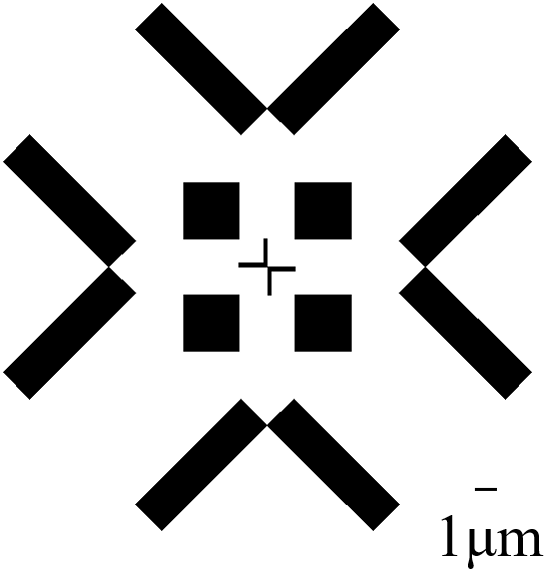
\includegraphics[width=10zw]{../images/mark.png}
\caption{�ʒu�����}�[�J�[}
\label{fig:mark}
\vspace*{1cm} % ����͂��܂��Ȃ��̂悤�Ȃ��̂ł��̂ŏ����Ă����Ă��������B

\includegraphics[width=12zw]{../images/mesa.png}
\caption{���T}
\label{fig:mark2}
\end{wrapfigure}
 \subsubsubsection{1.�ʒu�����p�}�[�J�[�쐻}
 PMMA��h�z���BEB�Ő}\ref{fig:mark}�̃p�^�[����`��㌻�����s�����B\\
 �d�q���������u��p����Ti(20nm),Au(180nm)�̏������s�����B\\
 ���̃p�^�[�����l���ɔz�u���邱�Ƃňȍ~�ł̍H����\\
 �`�摕�u�Ƃ̈ʒu�����Ńi�m�I�[�_�[�̐��x���o�����Ƃ��ł���B
 \subsubsubsection{2.���T�G�b�`���O}
 S1813��w�̃��W�X�g�ɂ��ALED�Ő}\ref{fig:mark2}�̃p�^�[����`���A\\
 �������s�����B�G�b�`���O�t�ɐZ���A�[����300nm�ɂȂ�悤��\\
 �G�b�`���O���s�����B���t�g�I�t��A�ēx���肷��Ɩ�270nm�������B
 \subsubsubsection{3.�u���b�W�̍쐻}
 �u���b�W�Ƃ͐}\ref{fig:superconductor}��(a)�A�̂悤�ɒ��`���d�ɂƃ{���f�B���O�p�b�h���q�������ł���B
 ���W�X�g��2�w��PMMA�ł���AEB�Ńp�^�[����`���A�������s�����B
 �d�q���������u��p����Ti(10nm),Au(90nm)�̏������s�����B
 \subsubsubsection{4.�I�[�~�b�N�R���^�N�g�̍쐻}
 ����͐}\ref{fig:superconductor}��(a)�B�̂悤�Ƀ��T�Ƃ̃R���^�N�g���Ƃ镔���ł���B
 LOR��S1813�̓�w�̃��W�X�g�ɂ��ALED�Ńp�^�[����`���A�������s�����B
 �󗰎_�����͂����ɒ�R���M���������u��p����AuGe(200nm),Ni(30nm)�̏������s�����B
 \subsubsubsection{5.�{���f�B���O�p�b�h�̍쐬}
 LOR��S1813�̓�w�̃��W�X�g�ɂ��ALED�Ő}\ref{fig:superconductor}��(a)�C�̂悤�Ƀp�^�[����`���A
 �������s�����B�󗰎_�����͂����ɓd�q���������u��p����Ti(20nm),Au(200nm)�̏������s�����B
 \subsubsubsection{6.���`���d�ɂ̍쐻}
 HEMT��‚̃��W�X�g��2�w��PMMA�ł���A�_�~�[��‚�LOR��S1813�̓�w�̃��W�X�g�ɂ��A
 EB�Ńp�^�[���̕`���A�������s�����B�󗰎_�����͂����ɓd�q���������u��p���Ă��ꂼ��̊�‚�
 �����̃p�^�[���̂�AuGe(40nm)�̏������s���A�����w��������Al,NbTi�̏������s�����B
 ���̒��`���p�^�[���͈�‚̃��T�ɑ΂���3�g��2�΂̒��`���d�ɂ�z�u���A���v��6�g�̒��`���d�ɂ��쐻�����B
 �}\ref{fig:superconductor}��(b),(c)�͑S�Ă̒��`���p�^�[����\���Ă���A���`���Ԃ̋�����(b)�̍�����
 2,0.3,0.6$\mu$m,(c)�̍�����0.6,2,2$\mu$m�ł���B
 \subsubsubsection{7.�A�j�[��}
 �A�j�[�����邱�ƂŁA���T�̃o�C�A�X���̓d�ɂƒ��d���d�ɂ�2�����d�q�n�Ƃ̃I�[�~�b�N�ȃR���^�N�g���Ƃ邱�Ƃ��ł���B
 \begin{figure}[htbp]
   \begin{center}
     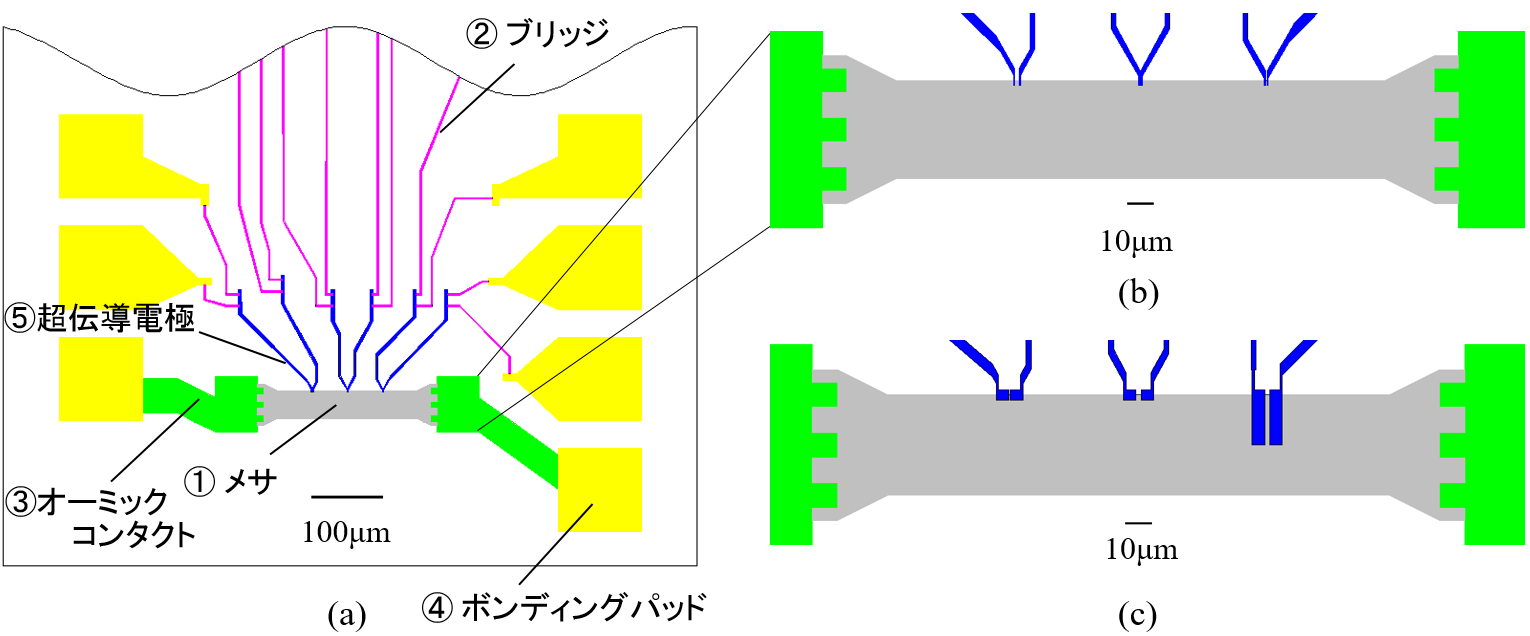
\includegraphics[width=18cm]{../images/superconductor.png}
   \end{center}
   \caption{���`���d��}
    \label{fig:superconductor}
 \end{figure}
%�쐬��‚̉摜�Ƃ��Ă͌����̑S�̊O�ςƃ_�~�[��‚̒��`���d�ɂƃA�j�[����̉摜
%HEMT��‚ł͓񎟌��d�q���̒��`���𑪒肷�邽�߂̃T���v����16�A\\
%�_�~�[��‚ł͎l�[�q����p�̃T���v����64�쐻�����B
\section{����n}
%��p�t�B���^
\end{document}

%\begin{thebibliography}{99}
%  \input{reference.txt}
%\end{thebibliography}


\appendix

\newpage
\printindex

\end{document}
